\scanpage{7}
\mspage{5}
Cette carte \inserted{$\mathcal X_2$} est déduite de $\mathcal X_0$ en faisant ``éclater'' les \deleted{\unsure{p}} sommets supersinguliers, ou encore de $\mathcal X_1$ en découpant \inserted{l'int.} des faces supersingulières et en identifiant des pts antipodiques sur leurs bords. --- ce qui explicite aussi la façon dont les $D_i$ sont plongés dans $\mathcal X$. Cette fois, on a une carte où toutes les faces peuvent être considérées comme \inserted{des $\unsure{\square}$} \deleted{d'}ordre \deleted{$\unsure{2n}$} $(4n)$, où tous les sommets d'ordre pair (et $=$ d'ordre $4$). Sur cette carte, les $\operatorname{Pol}(D)$ forment un syst. local (\deleted{mais} --- alors que sur $\mathcal X_0$, c'est ramifié (avec \uline{indice de ramification $n$}) autour de chaque sommet. Quant aux bouts libres, de part et d'autre de $D_i\subset\mathcal X$, ils se raccordent de façon satisfaisante encore. Cette carte d'autre part ne s'envoie \uline{pas} dans $X$ (sauf erreur).

\margin{\figure{%
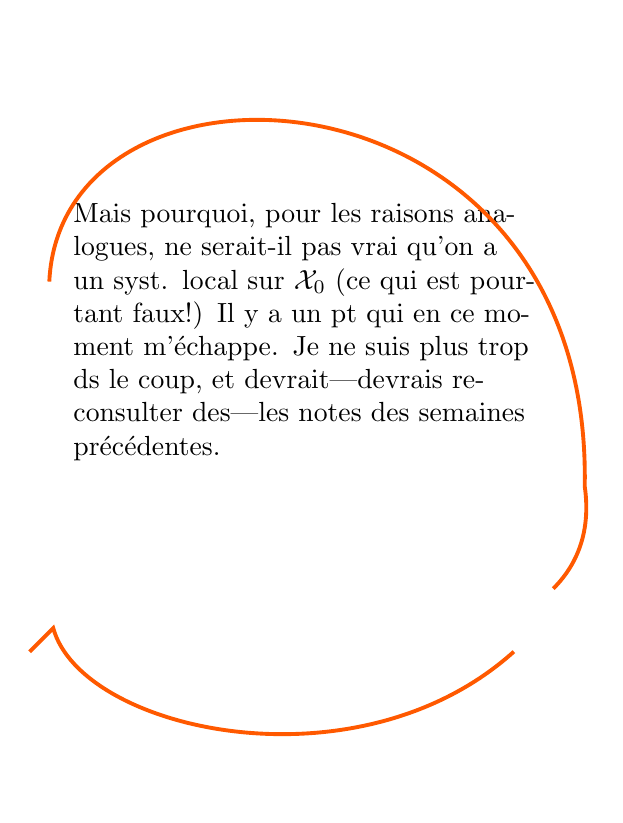
\begin{tikzpicture}[x=1cm,y=1cm]
\node[anchor=north west,text width=6.1cm,align=left,inner sep=0pt] at (0,0) {Mais pourquoi, pour les raisons analogues, ne serait-il pas vrai qu'on a un syst. local sur $\mathcal X_0$ (ce qui est pourtant faux!) Il y a un pt qui en ce moment m'échappe. Je ne suis plus trop ds le coup, et \unsure{devrait|devrais} reconsulter \unsure{des|les} notes des semaines précédentes.};
\draw[orange!70!red,line width=1.4pt] (-.3,-1)..controls(-.15,2.2)and(6.6,1.9)..(6.5,-3.6)..controls(6.6,-4.3)and(6.3,-4.7)..(6.1,-4.9);
\draw[orange!70!red,line width=1.4pt] (5.6,-5.7)..controls(3.6,-7.5)and(.1,-6.7)..(-.25,-5.4)--(-.55,-5.7);
\end{tikzpicture}%
}}

4) Ce dernier inconvénient n'est pas présent pour la carte $\mathcal X_3$, qui \deleted{est} par ailleurs
\margin{6}
